\documentclass[11pt, letterpaper, includehead]{article}

%%%%%%%%%%%%%%%%%%%%% Pre-document %%%%%%%%%%%%%%%%%%%%%
\usepackage{fancyhdr}
\usepackage{float}
\usepackage{array}
\usepackage{nicematrix}
\usepackage{enumitem}
\usepackage{titlesec}
\usepackage{multicol}
\usepackage{scrextend}
\usepackage{hyperref}
\usepackage{amssymb}
\usepackage{amsthm}
\usepackage{tikz}

\setlength{\parindent}{0pt} % Remove auto paragraph indents

% Get rid of those big margins
\usepackage[margin=1in]{geometry}
\newlength\titleindent
\setlength\titleindent{2cm}

\makeatletter
\def\@mathmargin{1in}
\makeatother

\titleformat{\section}[runin]
{\normalfont\bfseries}% formatting commands to apply to the whole heading
{\thesubsection}% the label and number
{0.5em}% space between label/number and subsection title
{}% formatting commands applied just to subsection title
[]% punctuation or other commands following subsection title

\theoremstyle{plain}

\newtheoremstyle{mydefinition}	% Name of the style
{} % Space above
{} % Space below
{\normalfont} % Body font (normal, not bold or italic)
{} % Indent amount
{\itshape} % Theorem head font (italic)
{.} % Punctuation after theorem head
{.5em} % Space after theorem head
{} % Theorem head spec (can be left empty)

\theoremstyle{mydefinition}
\newtheorem{defin}{Definition}

\newtheoremstyle{myproperty}  % Name of the style
{} % Space above
{} % Space below
{\normalfont} % Body font (normal, not bold or italic)
{} % Indent amount
{\itshape} % Theorem head font (italic)
{.} % Punctuation after theorem head
{.5em} % Space after theorem head
{} % Theorem head spec (can be left empty)

\theoremstyle{myproperty}
\newtheorem{prop}{Property}

\begin{document}

\pagestyle{fancy}
% Header
\fancyhead{}
\fancyhead[L]{\textbf{CS23:} Assignment \#5}
\fancyhead[R]{\href{mailto:stepanielh1111@gmail.com}{L'Heureux} \thepage}
% No page numbers for footer
\fancyfoot{}

\begin{center}
    \Large{\textbf{Assignment 5}}\\
    \Large{Trees and More Graphs}
\end{center}

\begin{enumerate}[label=\textbf{\arabic*}., leftmargin=*]
    \item We often define graph theory concepts using set theory. For example given a graph $G = (V, E)$ and a vertex $v \in V$, we define
    \[N(v) = \{ u \in V : \{v, u \} \in E\} \]
    We define $N[v] = N(v) \cup \{ v\} $. The goal of this problem is to figure out what all this means.

        
    \begin{enumerate}[label=(\alph*)]
        \item Let $G$ be the graph with $V = \{ a,b,c,d,e,f \} $ and
            \\$E = \{  \{ a,b \}, \{ a,e \},\{ b,c \}, \{ b,e \}, \{ c, d\}, \{ c, f\}, \{ d,f \}, \{ e,f \} \} $. 
            Find $N(a), N[a], N(c), \text{and} N[c]$.

                \[N(a) = \{b, e\}   \quad
                N[a] = \{a, b, e\}  \quad
                N(c) = \{b, d, f\}  \quad 
                N[c] = \{b, c, d, f\}\]
        \item What is the largest and smallest possible values for $|N(v)|$ and $|N[v]|$ for the graph from part (a)? Explain.
        
            $N(v)$ is the set of vertices incident to $v$, therefore: 
            \[|N(v)| = \deg(v)\]

            $N[v]$ is the set of vertices incident to $v$ union $v$ itself, therefore: 
            \[|N(v)| = \deg(v) + 1\]

            Given the degree sequence of the graph $G$ is:
            \[
            (2,\ 2,\ 3,\ 3,\ 3,\ 3)
            \]
            We compute the minimum and maximum values as follows:
            \[
            \min(|N(v)|) = 2 \quad \max(|N(v)|) = 3 \quad \min(|N[v]|) = 3 \quad \max(|N[v]|) = 4
            \]

        \item Give an example of a graph $G = (V, E)$ (Probably different from the one above) for which $N[v] = V$ for some vertex $v \in V$. Is there a graph for which $N[v] = V$ for \emph{all} $v \in V$? Explain.
        
        An example of a graph for which $N[v] = V$ for some $v \in V$ is any graph for which $v$ is adjacent to all other vertices in the graph. Example: \ref{fig:1c.G1}

        An example of a graph for which $N[v] = V$ for \emph{all} $v \in V$ is a graph in which for all $v \in V$, $v$ is adjacent to all other vertices. This is the case for any complete graph. Example: \ref{fig:1c.K6}.

        \begin{figure}[H]
            \centering
            \begin{minipage}[t]{0.45\textwidth}
                \centering
                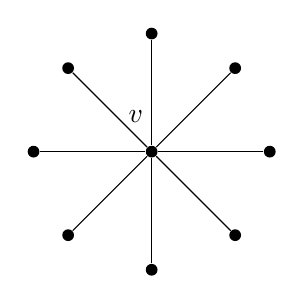
\begin{tikzpicture}[scale=1.5, every node/.style={circle, fill=black, inner sep=1.5pt}]
                    \foreach \i in {1,...,8} {
                        \node (N\i) at ({360/8* (\i - 1)}:1cm) {};
                    }
        
                    \node (N9) at (0,0) {};
                    \node[draw=none, fill=none, anchor=east] at (0, 0.3) {$v$};
        
                    \foreach \i in {1,...,8} {
                        \draw (N\i) -- (N9);
                    }
                \end{tikzpicture}
                \caption{$N[v] = V$ for $v \in V$}
                \label{fig:1c.G1}
            \end{minipage}
            \hfill
            \begin{minipage}[t]{0.45\textwidth}
                \centering
                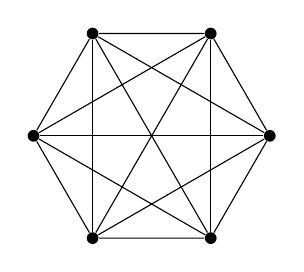
\begin{tikzpicture}[scale=1.5, every node/.style={circle, fill=black, inner sep=1.5pt}]
                    \foreach \i in {1,...,6} {
                        \node (N\i) at ({360/6 * (\i - 1)}:1cm) {};
                    }
        
                    \foreach \i in {1,...,5} {
                        \pgfmathtruncatemacro{\next}{\i+1}
                        \foreach \j in {\next,...,6} {
                            \draw (N\i) -- (N\j);
                        }
                    }
                \end{tikzpicture}
                \caption{$K_6$, $N[v] = V$ for all $v \in V$}
                \label{fig:1c.K6}
            \end{minipage}
        \end{figure}
        
        \item Give an example of a graph $G = (V, E)$ for which $N(v) = \emptyset$  for some $v \in V$. Is there an example of such graph for which $N[u] = V$ for some other $u \in V$ as well? Explain.
        
        An example of a graph for or which $N(v) = \emptyset$ for some $v \in V$ is any graph with an unconnected vertex $v$. Consider the example:
        \[G \text{ is a graph such that } V = \{a, b, c, d\} \text{ and } E = \{ \{a, b \}, \{b, c \}\} \text{ then } N(d) = \emptyset\]
        An example of such graph for which $N[u] = V$ for some other $u \in V$ as well does not exist. As discussed previously, for $N[u] = V$ for some $u \in V$, $u$ must be adjacent all other vertices in the graph. However, from the first part we know $v$ must be unconnected, and therefore $u$ cannot be adjacent to $v$. Thus, there exists no such graph.
        
        \item Describe in words what $N(v)$ and $N[v]$ mean in general.

        $N(v)$ is the set of vertices incident to $v$.\\
        $N[v]$ is the set of vertices incident to $v$ union $v$ itself.

    \end{enumerate}

    \item Which of the following graphs are trees
    \begin{enumerate}[label=(\alph*)]
        \item $G = (V, E)$ with $V = \{a, b, c, d, e\}$ and $E = \{ \{a, b \}, \{a, e \}, \{b, c \}, \{c, d \}, \{d, e\}\}$ 
        
        Not a tree--there exists a cycle.
        \item $G = (V, E)$ with $V = \{a, b, c, d, e\}$ and $E = \{ \{a, b \}, \{b, c \}, \{c, d \}, \{d, e \}\}$
        
        Tree.
        \item $G = (V, E)$ with $V = \{a, b, c, d, e\}$ and $E = \{ \{a, b \}, \{a, c \}, \{a, d \}, \{a, e \}\}$
        
        Tree (rooted tree).
        \item $G = (V, E)$ with $V = \{a, b, c, d, e\}$ and $E = \{ \{a, b \}, \{a, c \}, \{d, e \}\}$
        
        Not a tree--graph is disconnected. (However, there is a forest of two trees)
    \end{enumerate}

    \item For each degree sequence below, decide wether it must always, must never, or could possibly be a degree sequence for a tree. Remember, a degree sequence lists out the degrees (number of edges incident to the vertex) of all the vertices in a graph in non-increasing order.
    
        We know given a degree sequence, the number of edges is given by the Handshake Lemma:
        \[
            \sum_{v \in V} d(v) = 2e \quad \Rightarrow \quad e = \frac{1}{2} \sum_{v \in V} d(v)
        \]
        And tree always satisfies:
        \[e + 1 = v\]

    \begin{enumerate}[label=(\alph*)]
        \item $(4, 1, 1, 1, 1)$
        
        5 vertices, 4 edges. $v = e + 1$. Always a tree. 
        \item $(3, 3, 2, 1, 1)$

        5 vertices, 5 edges. $v \neq e + 1$ Not a tree.
        \item $(2, 2, 2, 1, 1)$
        
        5 vertices, 4 edges. $v = e + 1$. Possibly a tree.
        \item $(4, 4, 3, 3, 3, 2, 2, 1, 1, 1, 1, 1, 1, 1)$

        14 vertices, 14 edges. $v \neq e + 1$. Not a tree. 
    \end{enumerate}

    \item Suppose you have a graph with $v$ vertices and $e$ edges that satisfies $v = e + 1$. Must the graph be a tree? Prove your answer.
    \begin{proof} By counterexample

        Consider the graph $G = (V, E)$ with
        \[V = \{a, b, c, d\} \quad \text{and} \quad E = \{\{a, b\}, \{b, c\}, \{c, a\}\}\]

        In this case, $v = 4$ and $e = 3$, so the condition $v = e + 1$ holds:  
        \[4 = 3 + 1\]

        However, $G$ is not a tree. It contains a cycle between the vertices $a$, $b$, and $c$, which violates the definition of a tree. Furthermore, $G$ is disconnected, as vertex $d$ is isolated.

        While $G$ satisfies $v = e + 1$, it is not a tree.

        Therefore, if there exists a graph with $v$ vertices and $e$ edges that satisfies $v = e + 1$, it is not always a tree.
    \end{proof}

    \item Prove that any graph (not necessarily a tree) with $v$ vertices and $e$ edges that satisfies $v > e + 1$ will NOT be connected.

    \begin{proof} By contradiction

        Assume there exists a connected graph $G$ with $v$ vertices and $e$ edges that satisfies $v > e + 1$.
    
        We know every connected graph has a spanning tree. A spanning tree will have $v' = v$ vertices and $e' \leq e$ edges. 
        
        Thus the spanning tree will also have $v' > e' + 1$.

        But a tree must have $v = e + 1$, which is a contradiction, thus $G$ is not connected. 

        Therefore any graph with $v$ vertices and $e$ edges that satisfies $v > e + 1$ will NOT be connected.
    \end{proof}

    \item Let $T$ be a rooted tree that contains vertices $v, u, \text{ and } w$ (among possibly others). Prove that if $w$ is a descendant of both $u \text{ and } v$ then $u$ is a descendant of $v$ or $v$ is a descendant of $u$.
    
    \begin{proof} By contradiction

        Assume $w$ is a descendant of both $u \text{ and } v$ in a rooted tree.

        This implies that $w$ is not the root as it is a descendant of other vertices. Additionally, $u$ and $v$ are on a path from $w$ to the root by the definition of a descendant.

        By the definition of a rooted tree, there is exactly one simple path from any node to the root. Let the path from $w$ to the root be denoted by $P$.
    
        $P$ must either pass through both $u$ and $v$ or there exists another path to the root which would contradict the definition of a rooted tree.

        Therefore, either $u$ is a descendant of $v$ or $v$ is a descendant of $u$.    
    \end{proof}
    
    \item Prove that every connected graph which is not itself a tree must have at least three different spanning trees.

    \begin{proof} Direct proof

        Let $G$ be a connected graph which is not a tree.

        $G$ must therefore contain at least one cycle $C_n$ connecting some $n$ vertices.  

        To obtain a spanning tree we must remove an edge from the cycle $C_n$. Since the cycle contains $n$ edges, there are at least $n$ distinct ways to remove an edge and each may produce a unique spanning tree.

        Consider the minimum example in which $G$ contains only one cycle $C_3$. $C_3$ has three vertices and three edges. In this minimal case, there are three edges which can be removed, each producing a distinct spanning tree. 

        Therefore, every connected graph that is not itself a tree must have at least three distinct spanning trees.
    \end{proof}

\end{enumerate}

\end{document}